

\chapter{Estructura del proyecto}



Los Tribunales Ambientales son órganos jurisdiccionales especiales, sujetos a la 
superintendencia directiva, correccional y económica de la Corte Suprema, cuya función 
es resolver las controversias medioambientales de su competencia y ocuparse de los 
demás asuntos que la ley somete a su conocimiento \citet{Ley20600}. Estos tribunales generan una cantidad 
de jurisprudencia que puede ser encontrada en su portal de consulta llamado buscador ambiental \citet{BuscadorAmbiental}. 

El proyecto consiste en la generación de un chatbot en donde se pueda preguntar sobre 
la jurisprudencia de estos tribunales, aunque por razones de capacidad el chatbot se 
vea acotado solamente a las reclamaciones recibidas por el tribunal.

Por lo que, este proyecto consiste en un proceso de extracción de datos 
desde el buscador ambiental, transformación de estos datos para su utilización, generación 
de vectores de estos datos para que puedan interaccionar con la aplicación, carga de estos 
en una base de datos, para que después la aplicación pueda interactuar con ellos y mandando 
esa información a el LLM, siendo en este caso gpt-4 perteneciente a OpenAI.

% Inclusión de Figuras
\begin{figure}[ht!]
    \centering
    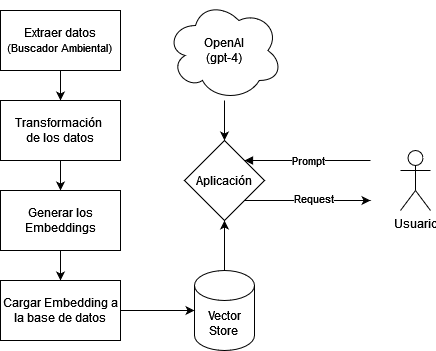
\includegraphics[width=.3\textwidth]{figures/huemul1.png}
    \caption[Estructura basica de la aplicación]{Estructura basica de la aplicación\\
    {\scriptsize (Fuente: Elaboración propia)}}
    \label{fig:logoind}
\end{figure}
    

A partir de esta estructura mientras se avance en el desarrollo, se explicará parte por parte el proceso y con ello los riesgos de cada uno de ellos.

